\documentclass[25pt, a1paper, portrait]{tikzposter}
\title{\parbox{0.8\linewidth}{\centering Repetitive Substructures for \\Efficient Representation of Automata}}
% \author{\vspace*{0.5em}Michal Šedý\vspace*{-0.5em}}
\author{\vspace*{1em}Michal Šedý}
\date{\today}
\institute{\normalsize supervised by doc. Mgr. Lukáš Holík, Ph.D.}

% Packages
\usepackage{url}
\usepackage{subfigure}
\usepackage{blindtext}
\usepackage{comment}
\usepackage{colortbl}
\usepackage{ctable}
\usepackage{tikz}
\usetikzlibrary{arrows,shapes,automata,backgrounds,petri,positioning}
\usetikzlibrary{decorations.pathmorphing}
\usetikzlibrary{decorations.shapes}
\usetikzlibrary{decorations.text}
\usetikzlibrary{decorations.fractals}
\usetikzlibrary{decorations.footprints}
\usetikzlibrary{shadows}
\usetikzlibrary{shapes.symbols}
\usetikzlibrary{shapes.callouts}
\tikzposterlatexaffectionproofoff


\usepackage{etoolbox}
\renewcommand\refname{}
\patchcmd{\thebibliography}{\section*{\refname}}{}{}{}


% Command for color circle around text.
\newcommand{\circledtext}[2][red]{%
    \tikz[baseline=(char.base)]{
        \node[shape=circle,draw=#1,fill=#1,inner sep=2pt] (char) {\hspace*{0.15mm}\textbf{#2}};}\hspace*{-2mm}
}

% Counter and environment for tables
\newcounter{tablecounter}
\newenvironment{tikztable}[1][]{%
  \def \rememberparameter{#1}%
  \refstepcounter{tablecounter}%
  \vspace{0.75em}}
  {
    \begin{center}
        \ifx\rememberparameter\@empty
        \else %nothing
        {\small Tab.~\thetablecounter: \rememberparameter \par\medskip}
        \fi
    \end{center}
}

% Set poster template
\usetheme{Envelope}
\useblockstyle[titleleft]{TornOut}
\colorlet{blocktitlefgcolor}{black!20!colorOne}
\usenotestyle{Sticky}

%%%%%%%%%%%%%%%%%%%%%%%%%%%%%%%%%%%%%%%%%%%%%%%%%%%%%%%%%%%%%%%%%%%%%%%%%%%%%%%
%%%%%%%%%%%%%%%%%%%%%%%%%%%%%%%%%%%%%%%%%%%%%%%%%%%%%%%%%%%%%%%%%%%%%%%%%%%%%%%
%%%%%%%%%%%%%%%%%%%%%%%%%%%%%%%%%%%%%%%%%%%%%%%%%%%%%%%%%%%%%%%%%%%%%%%%%%%%%%%
% DOCUMENT
%%%%%%%%%%%%%%%%%%%%%%%%%%%%%%%%%%%%%%%%%%%%%%%%%%%%%%%%%%%%%%%%%%%%%%%%%%%%%%%
%%%%%%%%%%%%%%%%%%%%%%%%%%%%%%%%%%%%%%%%%%%%%%%%%%%%%%%%%%%%%%%%%%%%%%%%%%%%%%%
%%%%%%%%%%%%%%%%%%%%%%%%%%%%%%%%%%%%%%%%%%%%%%%%%%%%%%%%%%%%%%%%%%%%%%%%%%%%%%%
\begin{document}

\maketitle[width=2\textwidth]

% Add logos
\node[below right=1cm and 11cm] at (TP@title) {
\includegraphics[width=0.28\textwidth]{images/excel-fit-2024-logo.pdf}};
\node[below left=1cm and 11cm] at (TP@title) {
\includegraphics[width=0.28\textwidth]{images/FIT_color_CMYK_EN.pdf}};

%%%%%%%%%%%%%%%%%%%%%%%%%%%%%%%%%%%%%%%%%%%%
%%%%%%%%%%%%%%%%%%%%%%%%%%%%%%%%%%%%%%%%%%%%
% MOTIVATION + PROCEDURES
%%%%%%%%%%%%%%%%%%%%%%%%%%%%%%%%%%%%%%%%%%%%
%%%%%%%%%%%%%%%%%%%%%%%%%%%%%%%%%%%%%%%%%%%%
\begin{columns}
    \column{0.4}
    \block{Motivation} {
        In many automata, especially those representing regular expressions, there exist repetitive substructures that cannot be eliminated by the state-of-the-art tool RABIT/Reduce \cite{RABIT}. Such an automaton is depicted below in Figure~\ref{fig:http}.

        \begin{tikzfigure}[\textsc{Network filtering automaton.}]
            \centering
            \begin{tikzpicture}[every initial by arrow/.style={, line width=1.5pt}, shorten >=1pt, node distance=3cm, auto, on grid, initial text=,font=\small,>=stealth',
                every state/.style={minimum size=7mm, line width=1.5pt}]
                \node[state, initial above , initial text=start] (0) {$0$};
                \node[cloud, line width=1.5pt, aspect=4, draw, cloud puffs=20, cloud puff arc=90, below left=4cm and 5cm of 0] (1) {\hspace*{-1.5em}\texttt{.*new XMLHttpRequest}\hspace*{-1.5em}};
                \node[cloud, line width=1.5pt, aspect=4, draw, cloud puffs=10, cloud puff arc=90, below right=4cm and 5cm of 0] (2) {\texttt{.*file://}};
                \node[state, below left=2.6cm and 5cm of 0, fill=orange] (11) {$\textbf{1}$};
                \node[state, below right=2.6cm and 5cm of 0, fill=white!50!blue] (22) {$\textbf{2}$};
                \node[state, below=2.8cm of 11, fill=orange] (33) {$\textbf{3}$};
                \node[state, below=2.8cm of 22, fill=white!50!blue] (44) {$\textbf{4}$};
                \node[cloud, line width=1.5pt, aspect=4, draw, cloud puffs=10, cloud puff arc=90, below=4.2cm of 33] (5) {\texttt{.*file://}};
                \node[cloud, line width=1.5pt, aspect=4, draw, cloud puffs=20, cloud puff arc=90, below=4.2cm of 44] (6) {\hspace*{-1.5em}\texttt{.*new XMLHttpRequest}\hspace*{-1.5em}};
                \node[state, below=2.8cm of 33, fill=white!20!red] (55) {$\textbf{5}$};
                \node[state, below=2.8cm of 44, fill=black!20!green] (66) {$\textbf{6}$};
                \node[state, below=2.8cm of 55, fill=white!20!red] (77) {$\textbf{7}$};
                \node[state, below=2.8cm of 66, fill=black!20!green] (88) {$\textbf{8}$};
                \node[state, accepting, below right=2.6cm and 5cm of 77] (9) {$9$};

                \path[->, line width=1.5pt]
                          (0) edge[out=west, in=north] node[above] {$\varepsilon$} (11)
                          (0) edge[out=east, in=north] node[above] {$\varepsilon$} (22)
                          (33) edge node[left] {$\varepsilon$} (55)
                          (44) edge node[right] {$\varepsilon$} (66)
                          (77) edge[out=south, in=west] node[below] {$\varepsilon$} (9)
                          (88) edge[out=south, in=east] node[below] {$\varepsilon$} (9);
            \end{tikzpicture}
            \label{fig:http}
        \end{tikzfigure}

        We propose a new method based on pushdown automata and so-called procedures that represent the repetitive substructures only once.
    }

    \note[
        rotate=12,
        targetoffsetx=6cm,
        targetoffsety=-11cm,
        width=0.125\linewidth
        ]
        {\small\textit{Usage of a pushdown automaton and procedures is an analogons to the call stack and functions from programming languages.}}

    \column{0.6}
    \block{One Procedure No Duplicate} {
        To represent automata efficiently without duplicate substructures, we introduce a new concept called procedures. Each redundant substructure is represented only once as a procedure. The automaton uses a stack to determine from which state the procedure is entered and to which state it should return. The symbol on the stack can also be used to guard transitions that are specific to only some substructures that the procedure represents.

        \begin{tikzfigure}[\textsc{Reduced network filtering automaton with two procedures.}]
            \centering
            \begin{tikzpicture}[every initial by arrow/.style={line width=1.5pt}, shorten >=1pt, node distance=3cm, auto, on grid, initial text=,font=\small,>=stealth',
                every state/.style={minimum size=7mm, line width=1.5pt}]
                \node[state, initial, initial text=start] (0) {$0$};
                \node[cloud, line width=1.5pt, aspect=6, draw, cloud puffs=30, cloud puff arc=90, above right=4cm and 9cm of 0] (1) {\texttt{.*new XMLHttpRequest}};
                \node[cloud, line width=1.5pt, aspect=4, draw, cloud puffs=30, cloud puff arc=90, below right=4cm and 9cm of 0] (2) {\texttt{.*file://}};
                \node[state, above right=4cm and 3.9cm of 0, fill=orange] (11) {$\textbf{1}$};
                \node[state, below right=4cm and 5.7cm of 0, fill=white!50!blue] (22) {$\textbf{2}$};
                \node[state, right=10.2cm of 11, fill=black!20!green] (33) {$\textbf{8}$};
                \node[state, right=6.6cm of 22, fill=white!20!red] (44) {$\textbf{7}$};
                \node[state, above right=1.2cm and 2cm of 22, fill=white!20!red] (66) {$\textbf{5}$};
                \node[state, above left=1.2cm and 2cm of 44, fill=white!50!blue] (88) {$\textbf{4}$};
                \node[state, above=5.6cm of 66, fill=orange] (55) {$\textbf{3}$};
                \node[state, above=5.6cm of 88, fill=black!20!green] (77) {$\textbf{6}$};
                \node[state, accepting, below right=4cm and 4.1cm of 33] (9) {$9$};
                \coordinate[above=1.5cm of 0] (0_1);
                \coordinate[below=1.5cm of 0] (0_2);
                \coordinate[above=1.5cm of 9] (3_9);
                \coordinate[below=1.5cm of 9] (4_9);
                \coordinate[below left=1.8cm and 0.3mm of 55] (5_6);
                \coordinate[above right=1.8cm and 0.3mm of 88] (8_7);


                \node[rectangle callout, draw, align=left, callout absolute pointer={($(0_1)-(0)$)}, above left=3cm and 2cm of 0] {\footnotesize\texttt{push(}\circledtext[orange]{1}\texttt{)}};
                \node[rectangle callout, draw, align=left, callout absolute pointer={($(4_9)-(0)$)}, below right=3cm and 2cm of 9] {\footnotesize\texttt{pop(}\circledtext[white!20!red]{5}\texttt{)}};
                \node[rectangle callout, draw, align=left, callout absolute pointer={($(0_2)-(0)$)}, below left=3cm and 2cm of 0] {\footnotesize\texttt{push(}\circledtext[white!50!blue]{2}\texttt{)}};
                \node[rectangle callout, draw, align=left, callout absolute pointer={($(3_9)-(0)$)}, above right=3cm and 2cm of 9] {\footnotesize\texttt{pop(}\circledtext[black!20!green]{6}\texttt{)}};

                \node[rectangle callout, draw, align=left, callout absolute pointer={($(5_6)-(0)$)}, below left=2.8cm and 3cm of 55] {\footnotesize\texttt{if top == }\circledtext[orange]{1}\texttt{:}\\[-1mm]\footnotesize\texttt{\hspace*{1em}pop(}\circledtext[orange]{1}\texttt{)}\\[-1mm]\footnotesize\texttt{\hspace*{1em}push(}\circledtext[white!20!red]{5}\texttt{)}};
                \node[rectangle callout, draw, align=left, callout absolute pointer={($(8_7)-(0)$)}, above right=2.8cm and 3cm of 88] {\footnotesize\texttt{if top == }\circledtext[white!50!blue]{2}\texttt{:}\\[-1mm]\footnotesize\texttt{\hspace*{1em}pop(}\circledtext[white!50!blue]{2}\texttt{)}\\[-1mm]\footnotesize\texttt{\hspace*{1em}push(}\circledtext[black!20!green]{6}\texttt{)}};


                \draw[->, line width=1.5pt, shorten >=1pt] (0) .. controls +(north:3cm) and +(west:2.7cm) .. (11);
                \draw[->, line width=1.5pt, shorten >=1pt] (0) .. controls +(south:3cm) and +(west:4.7cm) .. (22);
                \draw[->, line width=1.5pt, shorten >=1pt] (33) .. controls +(east:2.7cm) and +(north:3cm) .. (9);
                \draw[->, line width=1.5pt, shorten >=1pt] (44) .. controls +(east:4.7cm) and +(south:3cm) .. (9);
                \path[->, line width=1.5pt]
                          (55) edge[] node[left] {} (66)
                          (88) edge[] node[right] {} (77);
                \end{tikzpicture}
        \end{tikzfigure}
    }
\end{columns}

%%%%%%%%%%%%%%%%%%%%%%%%%%%%%%%%%%%%%%%%%%%%
%%%%%%%%%%%%%%%%%%%%%%%%%%%%%%%%%%%%%%%%%%%%
% EXPERIMENTS
%%%%%%%%%%%%%%%%%%%%%%%%%%%%%%%%%%%%%%%%%%%%
%%%%%%%%%%%%%%%%%%%%%%%%%%%%%%%%%%%%%%%%%%%%
\begin{columns}
    \column{0.5}
    \block{Parametric Regular Expressions}
    {
        We evaluated the reduction potential of procedures on 3,656 automata, with an average of 207 states and 2,584 transitions, generated from parametric regular expressions from \cite{Regex}.

        \begin{tikzfigure}[\textsc{The reduction ratios achieved by applying procedures to RABIT/Reduce results. On average, procedures improved reductions by 50.3\% in states and 47.9\% in transitions.}\par]
            \centering
            \begin{minipage}{0.21\textwidth}
                \centering
                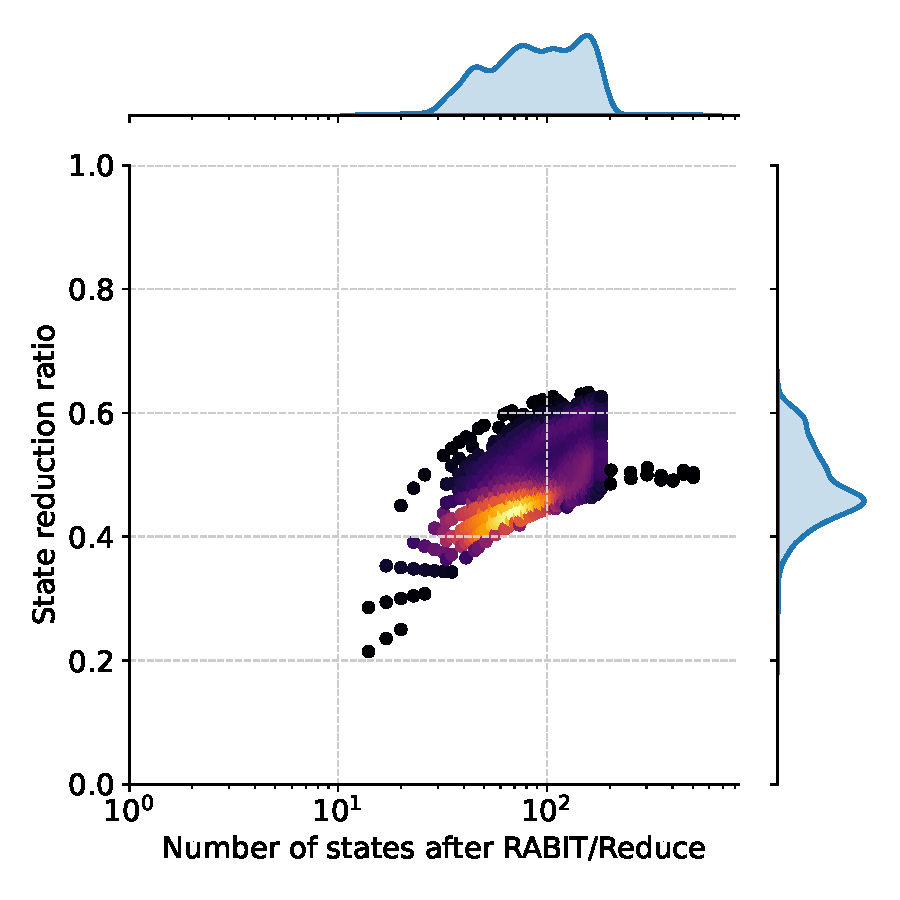
\includegraphics[width=1\linewidth]{images/intersect-all-states.pdf}
            \end{minipage}
            \begin{minipage}{0.21\textwidth}
                \centering
                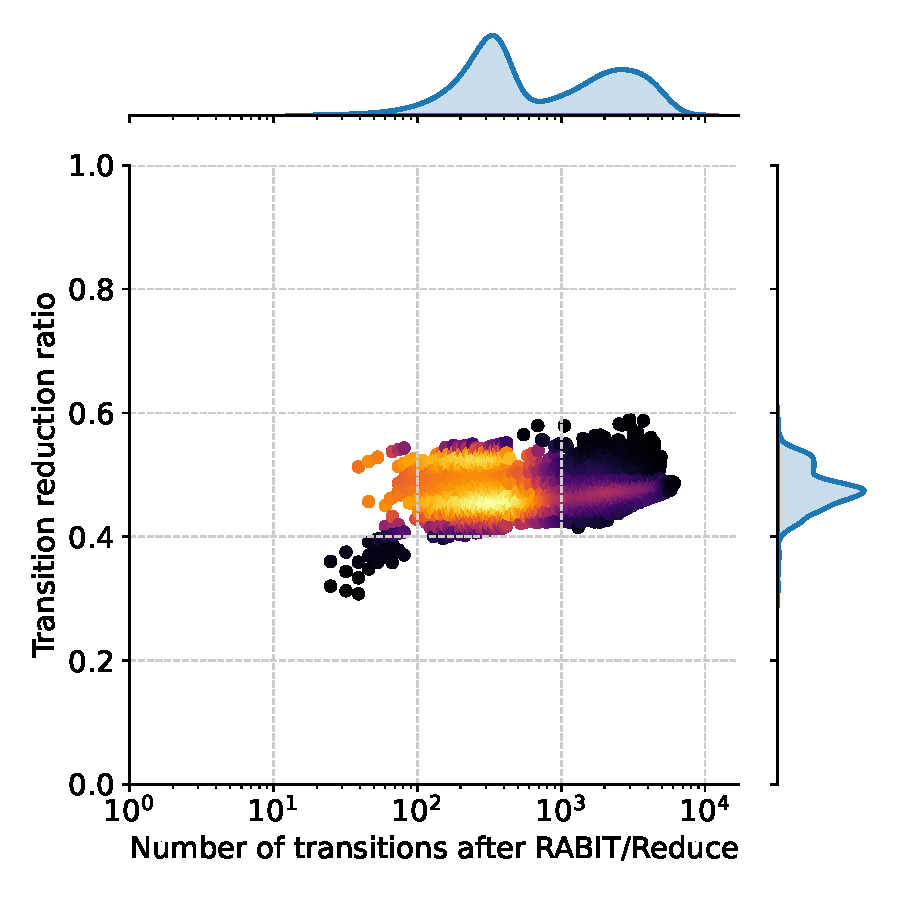
\includegraphics[width=1\linewidth]{images/intersect-all-trans.pdf}
            \end{minipage}
            \label{fig:regex}
        \end{tikzfigure}

        The standalone usage of RABIT/Reduce resulted on average in 52.5\% reduction of states and 48.4\% reduction of transitions. The further reduction performed by our algorithm can be seen in Figure \ref{fig:regex}. The application of procedures reduced the automata to half of the size given by RABIT/Reduce.
    }

    \column{0.5}
    \block[
        bodyoffsety=9cm,
        titleoffsety=9cm
      ]{Network Intrusion Detection System} {

        To test the reduction capability of procedures in a real-world scenario, we used rules from Snort (a well-known NIDS). We generated seven automata, each representing a union of regular expressions from a single category of Snort rules.

        \begin{tikztable}[\textsc{Reduction results of RABIT/Reduce (RAB) and procedures (Proc) on seven sets of Snort rules. $Q$ denotes the number of states $\delta$ the number of transitions, and $\Gamma$ the number of stack symbols. The percentages refer to the results of RABIT/Reduce.}\par]
            \centering
            \small
            \begin{tabular}{c|rr|rr|crrrr}
                Snort rules & \multicolumn{1}{c}{$Q_{in}$} & \multicolumn{1}{c|}{$\delta_{in}$} & \multicolumn{1}{c}{$Q_{RAB}$} & \multicolumn{1}{c|}{$\delta_{RAB}$} & \multicolumn{2}{c}{$Q_{Proc} + \Gamma_{Proc}$} & \multicolumn{2}{c}{$\delta_{Proc}$}\\
                \specialrule{.1em}{.05em}{.05em}
                p2p              & \hspace*{0.5em}33\hspace*{0.5em} &  1'090\hspace*{0.5em}   &\hspace*{0.5em} 32\hspace*{0.5em}   & 1'084\hspace*{0.5em}  & 25+6                   & (96.9\%) & \hspace*{0.5em}570    & (52.6\%)\\
                worm             & \hspace*{0.5em}50\hspace*{0.5em} &  3'880\hspace*{0.5em}   &\hspace*{0.5em} 34\hspace*{0.5em}     & 290\hspace*{0.5em}    & 24+8                  & (94.1\%)& \hspace*{0.5em}284    & (97.9\%)\\
                shellcode        & \hspace*{0.5em}162\hspace*{0.5em} & 3'328\hspace*{0.5em}   &\hspace*{0.5em} 56\hspace*{0.5em}     & 579\hspace*{0.5em}    & 48+2                 & (89.3\%) & \hspace*{0.5em}486    & (83.9\%)\\
                \rowcolor{yellow}mysql            & \hspace*{0.5em}235\hspace*{0.5em} & 30'052\hspace*{0.5em} & \hspace*{0.5em} 91\hspace*{0.5em}  & 14'430\hspace*{0.5em} & 45+18\hspace*{-0.5em}   & (69.2\%) & \hspace*{0.5em}7'142  & (49.5\%)\\
                chat             & \hspace*{0.5em}408\hspace*{0.5em} & 23'937\hspace*{0.5em} & \hspace*{0.5em}113\hspace*{0.5em}   & 1'367\hspace*{0.5em}  & 71+25\hspace*{-0.5em}  & (76.7\%) & \hspace*{0.5em}1'058  & (77.4\%)\\
                \rowcolor{yellow}specific-threats & \hspace*{0.5em}459\hspace*{0.5em} & 57'292\hspace*{0.5em} & \hspace*{0.5em}236\hspace*{0.5em}  & 31'935\hspace*{0.5em} & 99+32\hspace*{-0.5em}   & (55.5\%) & \hspace*{0.5em}12'680 & (39.7\%)\\
                telnet           & \hspace*{0.5em}829\hspace*{0.5em} & 7'070\hspace*{0.5em}  & \hspace*{0.5em}309\hspace*{0.5em}   & 2'898\hspace*{0.5em}  & 155+82                 & (50.0\%) & \hspace*{0.5em}2'164  & (74.7\%)\\
            \end{tabular}
            \normalsize
            \label{table:snort}
        \end{tikztable}

        The two most significant reductions are highlighted in Table~\ref{table:snort}. The best reduction was achieved on the automaton created from the \texttt{specific-threats} rule set. RABIT/Reduce reduced the automaton by 48.6\% of states and by 44.3\% of transitions. By further applying procedures, another 43.5\% reduction in states and 60.3\% reduction in transitions was achieved. This experiment demonstrates that procedures perform significant reductions even on real-world examples.
    }
    \block{References} {
        \vspace*{-2em}
        \small

        \bibliographystyle{enplain.bst}
        % \bibliographystyle{IEEEtran}
        \bibliography{bibliography}
        \normalsize
    }
\end{columns}

%%%%%%%%%%%%%%%%%%%%%%%%%%%%%%%%%%%%%%%%%%%%%%%%%%%%%%%%%%%%%%%%%%%%%%%%%%%%%%%
%%%%%%%%%%%%%%%%%%%%%%%%%%%%%%%%%%%%%%%%%%%%%%%%%%%%%%%%%%%%%%%%%%%%%%%%%%%%%%%
%%%%%%%%%%%%%%%%%%%%%%%%%%%%%%%%%%%%%%%%%%%%%%%%%%%%%%%%%%%%%%%%%%%%%%%%%%%%%%%
% DOCUMENT END
%%%%%%%%%%%%%%%%%%%%%%%%%%%%%%%%%%%%%%%%%%%%%%%%%%%%%%%%%%%%%%%%%%%%%%%%%%%%%%%
%%%%%%%%%%%%%%%%%%%%%%%%%%%%%%%%%%%%%%%%%%%%%%%%%%%%%%%%%%%%%%%%%%%%%%%%%%%%%%%
%%%%%%%%%%%%%%%%%%%%%%%%%%%%%%%%%%%%%%%%%%%%%%%%%%%%%%%%%%%%%%%%%%%%%%%%%%%%%%%
\end{document}
